\documentclass[conference,final]{IEEEtran}

\usepackage{latex8}
\usepackage{times}

\usepackage[utf8]{inputenc}
\usepackage{graphicx}
\usepackage{url}
\usepackage{float}
\usepackage{times}    
\usepackage{multirow}    
\usepackage{listings}   
\usepackage{times}     
\usepackage{paralist}    
\usepackage{wrapfig}    
\usepackage[small,it]{caption}
\usepackage{multirow}
\usepackage{ifpdf}


\usepackage{listings}
\usepackage{keyval}  
\usepackage{color}
\definecolor{listinggray}{gray}{0.95}
\definecolor{darkgray}{gray}{0.7}
\definecolor{commentgreen}{rgb}{0, 0.4, 0}
\definecolor{darkblue}{rgb}{0, 0, 0.4}
\definecolor{middleblue}{rgb}{0, 0, 0.7}
\definecolor{darkred}{rgb}{0.4, 0, 0}
\definecolor{brown}{rgb}{0.5, 0.5, 0}

\lstdefinestyle{myListing}{
  frame=single,   
  backgroundcolor=\color{listinggray},  
  %float=t,
  language=C,       
  basicstyle=\ttfamily \footnotesize,
  breakautoindent=true,
  breaklines=true
  tabsize=2,
  captionpos=b,  
  aboveskip=0em,
  belowskip=-2em,
  %numbers=left, 
  %numberstyle=\tiny
}      

\lstdefinestyle{myPythonListing}{
  frame=single,   
  backgroundcolor=\color{listinggray},  
  %float=t,
  language=Python,       
  basicstyle=\ttfamily \footnotesize,
  breakautoindent=true,
  breaklines=true
  tabsize=2,
  captionpos=b,  
  %numbers=left, 
  %numberstyle=\tiny
}

\newcommand{\up}{\vspace*{-1em}}
\newcommand{\upp}{\vspace*{-0.5em}}
\newcommand{\numrep}{16 }
\newcommand{\samplenum}{4 }
\newcommand{\tmax}{$T_{max}$ }
\newcommand{\tc}{$T_{C}$ }

\title{SAGA-based BigJob: A pervasive, general purpose Pilot-Job Abstraction for Distributed Systems}

\author{
Andr\'e Luckow$^{1}$, Lukasz Lacinski$^{1}$,   Shantenu Jha$^{1,2,3,*}$,\\
  \small{\emph{$^{1}$Center for Computation \& Technology, Louisiana State University, USA}}\\
  \small{\emph{$^{2}$Department of Computer Science, Louisiana State University, USA}}\\
  \small{\emph{$^{3}$e-Science Institute, Edinburgh, UK}}\\
  \small{\emph{$^{*}$Contact Author: \texttt{sjha@cct.lsu.edu}}}\\
}

%\date{}

\def\acknowledgementname{Acknowledgements}
\newenvironment{acknowledgement}%
{\section*{\acknowledgementname}%
\parindent=0pt%
}

\newif\ifdraft
% \drafttrue
\ifdraft
\newcommand{\llnote}[1]{ {\textcolor{green} { ***JK: #1 }}}
\newcommand{\alnote}[1]{ {\textcolor{blue} { ***AL: #1 }}}
\newcommand{\jhanote}[1]{ {\textcolor{red} { ***SJ: #1 }}}
\else
\newcommand{\llnote}[1]{}
\newcommand{\alnote}[1]{}
\newcommand{\jhanote}[1]{}
\fi

\begin{document} 

\maketitle    

% \up\up\up\up

\begin{abstract}
The uptake of distributed infrastructure by scientific applications has been limited by the availability of extensible, pervasive and simple to use abstractions. Effective abstractions are required at multiple levels -- development, deployment and execution stages of scientific applications. The Pilot-Job abstraction has been 
shown to be an effective abstraction to address many requirements of scientific applciations. Howeever there are multiple Pilot-Job abstractions which are often tied to a specific infrastructure.  In this paper, we introduce a SAGA-based Pilot-Job which supports a wide range of application types and is usable over a broad range of infrastructure, i.e. is both general-purpose and pervasive.  Emerging distributed infrastructure such as Clouds provide different resource provisioning models from classical Grids. This introduces new opportunities for distributed applications and the support of dynamical execution models. In this paper, we discuss how the
SAGA-based Pilot-Job has been used for different application types and supports concurrent usage across
multiple heterogeneous distributed infrastructure.
\end{abstract}

% \up \up
\Section{Introduction}
% \up

Several classes of applications are well suited for distributed
environments. Probably the best known and most powerful examples are
those that involve an ensemble of decoupled tasks, such as simple
parameter sweep applications~\cite{1239909}.

\emph{Pilot jobs} is a concept initially pioneered by Condor Glide-In, which
has been used by many communities to increase the predictability
and time-to-solution of such applications. A pilot job allows the execution 
of jobs which the necessity to queue each individual sub-job. The pilot job itself
is a regular Grid job, which is started through a Grid resource manager, such as
the Globus GRAM.

The Simple API for Grid Applications (SAGA) is a high-level, easy-to-use API for 
accessing distributed resources. Unlike other common pilot job systems SAGA BigJob 
(i) natively supports MPI job and (ii) works on a variety of back-end systems, 
generally reflecting the advantage of using a SAGA-based approach.

Discuss PilotJob:
- How Traditionally Used (mostly deployment time)
- How traditionally bound to a single platform and system

Recently, the usage of virtualization and the usage of on-demand virtual machines
become increasingly popular. These so-called infrastructure-as-a-service clouds have
different advantages compared to traditional Grid systems: users are provided
with a greater flexibility and have the ability to customize their virtual machine
environment. At the same time virtual machines are well isolated from each other. More and
more the need to integrate traditional Grids and Clouds arises.

%from autonomic HPC Grid/Cloud paper
Developing and running applications in such a hybrid and dynamic computational 
infrastructure presents new and significant challenges. These include the need for programming 
systems that can express the hybrid usage modes and associated runtime trade-offs and adaptations, 
as well as coordination and management infrastructures that can implement them in an efficient 
and scalable manner. Key issues include decomposing applications, components and workflows, 
determining and provisioning the appropriate mix of Grid/Cloud resources, and dynamically scheduling 
them across the hybrid execution environment while satisfying/balancing multiple, possibly changing 
objectives for performance, resilience, budgets and so on.


\Section{Related Work}

Condor Glide-In

Falkon

Nimbus

CERN Atlas Pilot Job~\cite{1555338}

\Section{BigJob -- The SAGA-based Pilot Job}

Introduce BigJob:
 - Describe it, and how it differs from other PilotJobs

 - Outline new usage modes that BigJob fundamentally supports:
    -- As the basis for scale-out across
    -- As the basis for a framework for runtime optimization
    -- More thought?

BigJob:
 - Architecture and control flow details
 - Performance Numbers

\SubSection{Overview}


The following figure gives an overview of the SAGA BigJob architecture.

\begin{figure}[htbp]
    \centering
    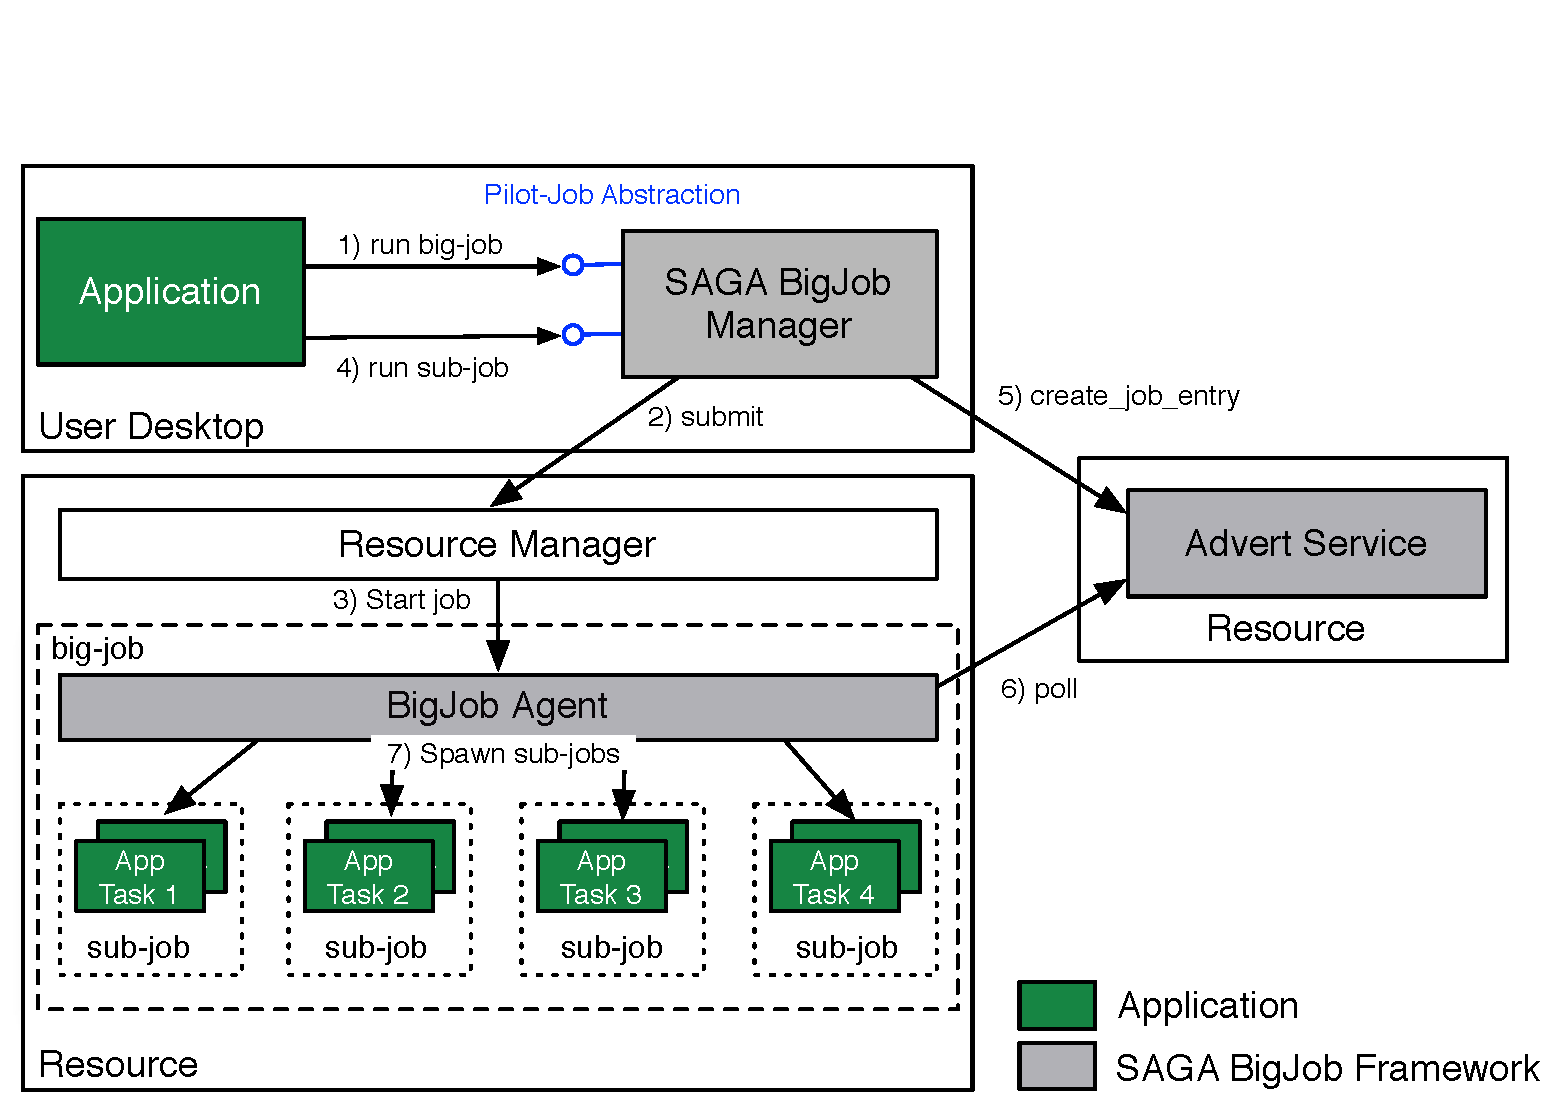
\includegraphics[width=0.45\textwidth]{figures/bigjob}
    \caption{BigJob Architecture: The core of the framework, the BigJob-Manager,
     orchestrates a set of BigJob-Agents and sub-jobs using the SAGA job and file APIs. 
     The BigJob-Agent is responsible for managing and monitoring sub-jobs on a 
     single machine.}
    \label{fig:figures_bigjob}
\end{figure}


\SubSection{Performance}

Startup Times

Dispatch times


\Section{BigJob for Utilizing Cloud Resources}

Despite a standardized interface, big difference on how to obtain meta-data (internal ip etc.)

OCCI

\section{Usage Modes and Analaysis}

The aim of this section is not to perform detailed systematic
performance measures and analysis, but to illustrate the various usage
modes the SAGA-based BigJob can support and how they are supported. We
posit that the performance overheads of BigJob are small relative to
the duration of the tasks that are typically performed, i.e., order of
seconds compared to tens of minutes and hours.  Needless to say, if
millions of jobs each of short duration were being attempted then the
overheads would be significant.

We discuss two scenarios that are representative of how applications
would typically use multiple distributed infrastructure. We focus our
attention on replica-based MD simulations and define a workload as
\numrep replicas of the HCV model~\cite{}, each replica running for
500 timesteps.  The first scenario involves running all \numrep over
different infrastructure configurations and determining the \tc for
each scenario. We repeat \tc for each configuration \samplenum times.

The second scenario, introduces an upper-bound on the acceptable \tc
(defined as \tmax) -- which is the maximum permissible time to
solution.

Each scenario has several possible specific sub-scenarios, of which we
discuss a few in each.

\subsection{List and explain the resources used in Experiments}

\subsubsection*{Resource I: TeraGrid/LONI Cluster (QB)}

\subsubsection*{Resource II: Condor-Pool of LONI Clusters}

\jhanote{This one will require most description -- how the pool is set
up, what features are used etc}

\subsubsection*{Resource III: Cloud Environments}


\subsection{Scenario I: \tc for Workload for Different Resource Configurations}

\subsubsection{\tc for single Resource Usage}

\subsubsection{\tc for Collective Resource Utilization}

\begin{itemize}
\item Resource I and III:
\item Resource II and III:
\item Resource I, II and III:
\end{itemize}

\subsection{Scenario II: Investigation of the Distribution of Workload for Maximum Allowed
  Time to Solution} 

Given that Clouds provide the illusion of infinite capacity, or at
least queue wait-times are non-existent, it is likely that often most
sub-jobs will end up on the Cloud infrastructure.  Thus in Scenario
II, the resource assignment algorithm we use is as follows: We submit
tasks to non-cloud resource first, and if the jobs have not finished
when time equal to $T_{X}$ (defined as: \tmax - 2 average \tc on all
clouds) has elapsed, than we move the workload to utilize clouds.  The
underlying basis is that clouds have an explit cost associated with
them and if jobs can be completed on the the TG and Condor pool while
preserving the performance constraints, we opt for such a
solution. However, if queue loads prevent the performance requirements
being met, we move the jobs to a cloud-resource, which we have shown
has less fluctuation in \tc of the workload.

\subsection{Case Study: Running BigJob Across Heterogeneous Infrastructures}

NAMD

No discovery service - it is more or less a surprise what kind of capabilities you get in each science cloud

Test new Amazon High Memory Machine

Eucalyptus networking completely screwed up: all images start with the same hostname

Images not transferable

Different feature set

\Section{Conclusion}

We plan to extend this work in two important directions. The first is
the use of a more sophisticated coordination mechanism -- that
supports asynchronous task coordination (e.g., Comet). In this paper,
we have focussed on replica simulations, but not on replica-exchange
simulations -- which involve coordination between the different tasks
and intelligence in their placements.  It will be very interesting to
note the performance gains that accrue as a result of such
asynchronous coordination on production infrastructure for the
replica-exchange problems. Also, having established the basic
infrastructure to submit tasks to and manage multiple, heterogenous
resources using a simple, single interface, an important second
extension of this work is to use more sophisticated task-placement
decisions or resource utilization decision making.

\end{document}
